% figures.tex — Tables and figures for INSTRUMENTAL paper

% ─────────────────────────────────────────────────────────────
% Table 1: Results progression
% ─────────────────────────────────────────────────────────────
\begin{table}[H]
\centering
\caption{Progression of synthesizer parameter recovery across key development versions. Each row marks a milestone where a qualitative improvement was introduced.}
\label{tab:progression}
\begin{tabular}{@{}lcrl@{}}
\toprule
\textbf{Version} & \textbf{Params} & \textbf{Loss} & \textbf{Key Change} \\
\midrule
v5  & 15 & 4.60 & Basic pipeline \\
v11 & 18 & 2.34 & CMA-ES + initialization \\
v22 & 24 & 2.13 & + pulse width \& slope \\
v24 & 28 & 2.09 & + parametric EQ \\
\bottomrule
\end{tabular}
\end{table}

% ─────────────────────────────────────────────────────────────
% Table 2: Hypothesis testing
% ─────────────────────────────────────────────────────────────
\begin{table}[H]
\centering
\caption{Ablation study over synthesizer component hypotheses. Each row shows the loss when the given component is added or removed. The best-performing configuration (parametric EQ) is highlighted.}
\label{tab:hypotheses}
\begin{tabular}{@{}lrr@{}}
\toprule
\textbf{Hypothesis} & \textbf{Loss} & \textbf{Change (\%)} \\
\midrule
Baseline (v22)            & 2.13 &  ---   \\
Remove slope parameter    & 2.28 & +7.0  \\
Remove pulse width        & 2.19 & +2.8  \\
Double population size     & 2.12 & $-$0.5 \\
Halve population size      & 2.18 & +2.3  \\
Add noise oscillator       & 2.15 & +0.9  \\
Add sub-oscillator         & 2.14 & +0.5  \\
\textbf{Add parametric EQ} & \textbf{2.09} & $\mathbf{-1.9}$ \quad{\color{green!60!black}$\boldsymbol{\checkmark}$} \\
\bottomrule
\end{tabular}
\end{table}

% ─────────────────────────────────────────────────────────────
% Figure 1: Convergence curve
% ─────────────────────────────────────────────────────────────
\begin{figure}[H]
\centering
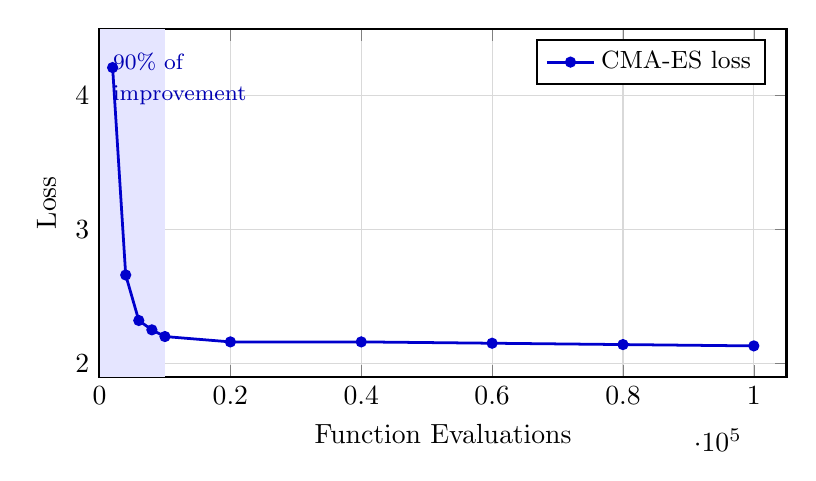
\begin{tikzpicture}
\begin{axis}[
    width=0.85\linewidth,
    height=6cm,
    xlabel={Function Evaluations},
    ylabel={Loss},
    xmin=0, xmax=105000,
    ymin=1.9, ymax=4.5,
    xtick={0,20000,40000,60000,80000,100000},
    xticklabel style={/pgf/number format/fixed, /pgf/number format/1000 sep={\,}},
    grid=major,
    grid style={gray!30},
    legend pos=north east,
    legend style={font=\small},
    thick,
]
% Shaded region: first 10K evals = 90% of improvement
\fill[blue!10] (axis cs:0,1.9) rectangle (axis cs:10000,4.5);
\node[anchor=north west, font=\footnotesize, text=blue!70!black] at (axis cs:500,4.4) {90\% of};
\node[anchor=north west, font=\footnotesize, text=blue!70!black] at (axis cs:500,4.15) {improvement};

\addplot[
    color=blue!80!black,
    mark=*,
    mark size=1.5pt,
    line width=1pt,
] coordinates {
    (2000,4.21)
    (4000,2.66)
    (6000,2.32)
    (8000,2.25)
    (10000,2.20)
    (20000,2.16)
    (40000,2.16)
    (60000,2.15)
    (80000,2.14)
    (100000,2.13)
};
\addlegendentry{CMA-ES loss}
\end{axis}
\end{tikzpicture}
\caption{Convergence of CMA-ES optimization over function evaluations. The shaded region highlights the first 10{,}000 evaluations, within which approximately 90\% of total loss reduction is achieved.}
\label{fig:convergence}
\end{figure}

% ─────────────────────────────────────────────────────────────
% Figure 2: Pipeline flowchart
% ─────────────────────────────────────────────────────────────
\begin{figure}[H]
\centering
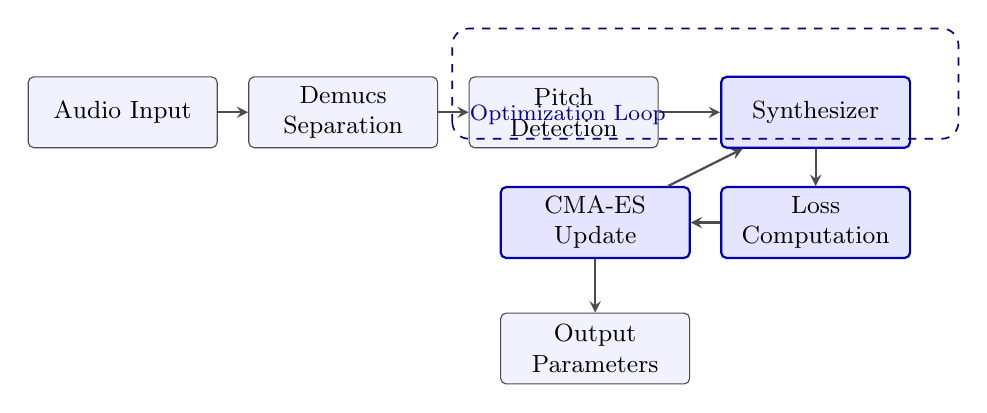
\begin{tikzpicture}[
    node distance=1.6cm,
    box/.style={
        rectangle, draw=black!70, fill=blue!5,
        minimum width=2.4cm, minimum height=0.9cm,
        align=center, rounded corners=2pt,
        font=\small
    },
    loopbox/.style={
        rectangle, draw=blue!70!black, fill=blue!10,
        minimum width=2.4cm, minimum height=0.9cm,
        align=center, rounded corners=2pt,
        font=\small, line width=0.8pt
    },
    arr/.style={->, >=stealth, thick, black!70},
]
% Nodes
\node[box] (audio) {Audio Input};
\node[box, right of=audio, node distance=2.8cm] (demucs) {Demucs\\Separation};
\node[box, right of=demucs, node distance=2.8cm] (pitch) {Pitch\\Detection};

% CMA-ES loop
\node[loopbox, right of=pitch, node distance=3.2cm] (synth) {Synthesizer};
\node[loopbox, below of=synth, node distance=1.4cm] (loss) {Loss\\Computation};
\node[loopbox, left of=loss, node distance=2.8cm] (update) {CMA-ES\\Update};

% Output
\node[box, below of=update, node distance=1.6cm] (output) {Output\\Parameters};

% Arrows
\draw[arr] (audio) -- (demucs);
\draw[arr] (demucs) -- (pitch);
\draw[arr] (pitch) -- (synth);
\draw[arr] (synth) -- (loss);
\draw[arr] (loss) -- (update);
\draw[arr] (update) -- (synth);
\draw[arr] (update) -- (output);

% Loop label
\draw[dashed, blue!50!black, rounded corners=6pt, line width=0.6pt]
    ([xshift=-0.6cm, yshift=0.6cm]update.north west) rectangle
    ([xshift=0.6cm, yshift=0.6cm]synth.north east);
\node[font=\footnotesize, blue!60!black, anchor=south west]
    at ([xshift=-0.5cm, yshift=0.65cm]update.north west) {Optimization Loop};

\end{tikzpicture}
\caption{End-to-end pipeline for synthesizer parameter recovery. The input audio is separated using Demucs, followed by pitch detection. CMA-ES iteratively synthesizes candidate audio, computes a perceptual loss against the target, and updates the parameter vector until convergence.}
\label{fig:pipeline}
\end{figure}

% ─────────────────────────────────────────────────────────────
% Figure 3: Harmonic amplitude comparison
% ─────────────────────────────────────────────────────────────
\begin{figure}[H]
\centering
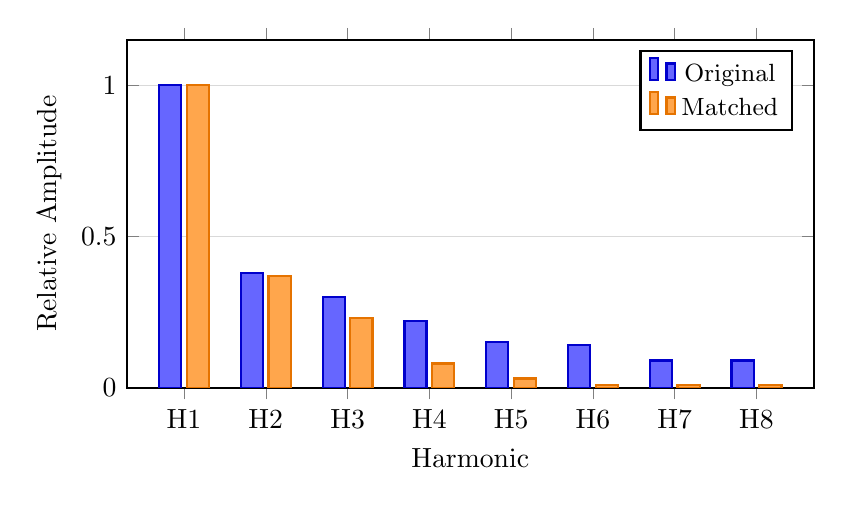
\begin{tikzpicture}
\begin{axis}[
    width=0.85\linewidth,
    height=6cm,
    ybar,
    bar width=8pt,
    xlabel={Harmonic},
    ylabel={Relative Amplitude},
    ymin=0, ymax=1.15,
    xtick=data,
    xticklabels={H1, H2, H3, H4, H5, H6, H7, H8},
    enlarge x limits=0.1,
    grid=major,
    grid style={gray!30},
    ymajorgrids=true,
    xmajorgrids=false,
    legend pos=north east,
    legend style={font=\small},
    thick,
]
\addplot[fill=blue!60, draw=blue!80!black] coordinates {
    (1,1.0) (2,0.38) (3,0.30) (4,0.22) (5,0.15) (6,0.14) (7,0.09) (8,0.09)
};
\addlegendentry{Original}

\addplot[fill=orange!70, draw=orange!90!black] coordinates {
    (1,1.0) (2,0.37) (3,0.23) (4,0.08) (5,0.03) (6,0.01) (7,0.01) (8,0.01)
};
\addlegendentry{Matched}
\end{axis}
\end{tikzpicture}
\caption{Comparison of harmonic amplitudes between the original audio and the synthesizer output matched via CMA-ES. The first three harmonics are closely reproduced, while higher-order harmonics (H4--H8) show greater divergence.}
\label{fig:harmonics}
\end{figure}
